\documentclass[12pt,a4,UTF8]{article}




\usepackage{graphicx,amsmath,amssymb,amsthm, boxedminipage,xcolor,amscd,amsbsy,latexsym,url,bm}

%\usepackage[lined,boxed]{algorithm2e}

\usepackage{algorithm}
\usepackage{algpseudocode}


\newtheorem{theorem}{Theorem}[section]
\newtheorem{proposition}[theorem]{Proposition}
\newtheorem{lemma}[theorem]{Lemma}
\newtheorem{corollary}[theorem]{Corollary}
\newtheorem{definition}[theorem]{Definition}

\newtheorem*{theorem*}{Theorem}
\newtheorem*{lemma*}{Lemma}
\newtheorem*{solution}{Solution}
\newtheorem*{proposition*}{Proposition}


\newtheorem{exercise}[theorem]{Exercise}
\newtheorem{exerciseD}[theorem]{*Exercise}
\newtheorem{exerciseDD}[theorem]{**Exercise}

\let\oldexercise\exercise
\renewcommand{\exercise}{\oldexercise\normalfont}

\let\oldexerciseD\exerciseD
\renewcommand{\exerciseD}{\oldexerciseD\normalfont}

%\let\oldexerciseD\exerciseD
%\renewcommand{\exerciseD}{\oldexerciseD\normalfont}

%\let\oldexerciseDD\exerciseDD
%\renewcommand{\exerciseDD}{\oldexerciseDD\normalfont}

\newcommand{\E}{\mathbb{E}}
%\newcommand{\nth}[1]{#1^{\textsuperscript{th}}}
\newcommand{\scalar}[2]{\ensuremath{\langle #1, #2\rangle}}
\newcommand{\floor}[1]{\left\lfloor #1 \right\rfloor}
\newcommand{\ceil}[1]{\left\lceil #1 \right\rceil}
\newcommand{\norm}[1]{\|#1\|}
\newcommand{\pfrac}[2]{\left(\frac{#1}{#2}\right)}
\newcommand{\nth}[1]{#1^{\textsuperscript{th}}}
\newcommand{\core}{\textnormal{core}}



\newif\ifsolution

\solutionfalse

\newcommand{\answer}[1]{
\ifsolution
{\color{blue} #1}
\else
\fi
}



\newcommand{\poly}{\textnormal{poly}}
\newcommand{\quasipol}{\textnormal{quasipol}}
\newcommand{\ssubexp}{\textnormal{stronglySubExp}}
\newcommand{\wsubexp}{\textnormal{weaklySubExp}}
\newcommand{\simplyexp}{\textnormal{E}}
\newcommand{\expo}{\textnormal{Exp}}



\newcommand{\N}{\mathbb{N}}
\newcommand{\nn}{\mathbb{N}_0^n}
\newcommand{\R}{\mathbb{R}}
\newcommand{\Z}{\mathbb{Z}}


\definecolor{darkgreen}{rgb}{0,0.6,0}

\date{}

\title{
\hbox{  Mathematical Foundations of Computer Science}
  \vspace{3mm}
{\normalsize CS 499,	Shanghai Jiaotong University,  Dominik Scheder\\
%\vspace{3mm}
Spring 2019}
}


\begin{document}

\maketitle

%\begin{quotation}
%  You are welcome to discuss the exercises in the discussion
%  forum. Please take them serious. Doing the exercises is as important
%  than watching the videos.
%
%  I intentionally included very challenging exercises and marked them
%  with one or two ``$*$''. No star means you should be able to solve
%  the exercises without big problems once you have understood
%  the material from the video lecture. One star means it requires 
%  significant additional thinking. Two stars means it is not 
%  unlikely that you will fail to solve them, even once you have understood
%  the material and thought a lot about the exercise. Don't feel bad
%  if you fail. Failure is part of learning.
%
%  This is the first time this course is online. Thus there might be mistakes
%  (typos or more serious conceptual mistakes) in the exercises. I will be 
%  grateful if you point them out to me!
%\end{quotation}





\setcounter{section}{5}
\begin{center}
  \large\textbf{Group: navigator} 
\end{center}
\begin{center}
  \begin{tabular}{rl}
 Xu Huan  & 517021910724 \\
 Tianyao Shi     &     517021910623 \\
Chenxiao Yang    &    517021910540  \\
Jiaqi  Zeng      &     517021910882  \\
  \end{tabular}
\end{center}
\newpage

\section{Graph Automorphisms}


Let $G = (V, E)$ and $H = (V', E')$ be two graphs. A {\em graph isomorphism} from $G$ to $H$
 is a bijective function $f: V \rightarrow V'$ such that
 for all $u,v \in V$ it holds that $\{u,v\} \in E$ if and only if $\{f(u),f(v)\} \in E'$. 
 If such a function exists, we write $G \cong H$ and say that $G$ and $H$ are {\em isomorphic}.
 In other words, $G$ and $H$ being isomorphic means that they 
 are identical up to the names of its vertices.
 
Obviously, every graph $G$ is isomorphic to itself, because the identity function $f(u) = u$ is an
isomorphism. However, there might be several isomorphisms $f$ from $G$ to $G$ itself.
We call such an isomorphism from $G$ to itself an {\em automorphism} of $G$.

\begin{exercise}
For each of the graphs below, compute the number of automorphisms it has.
\begin{center}
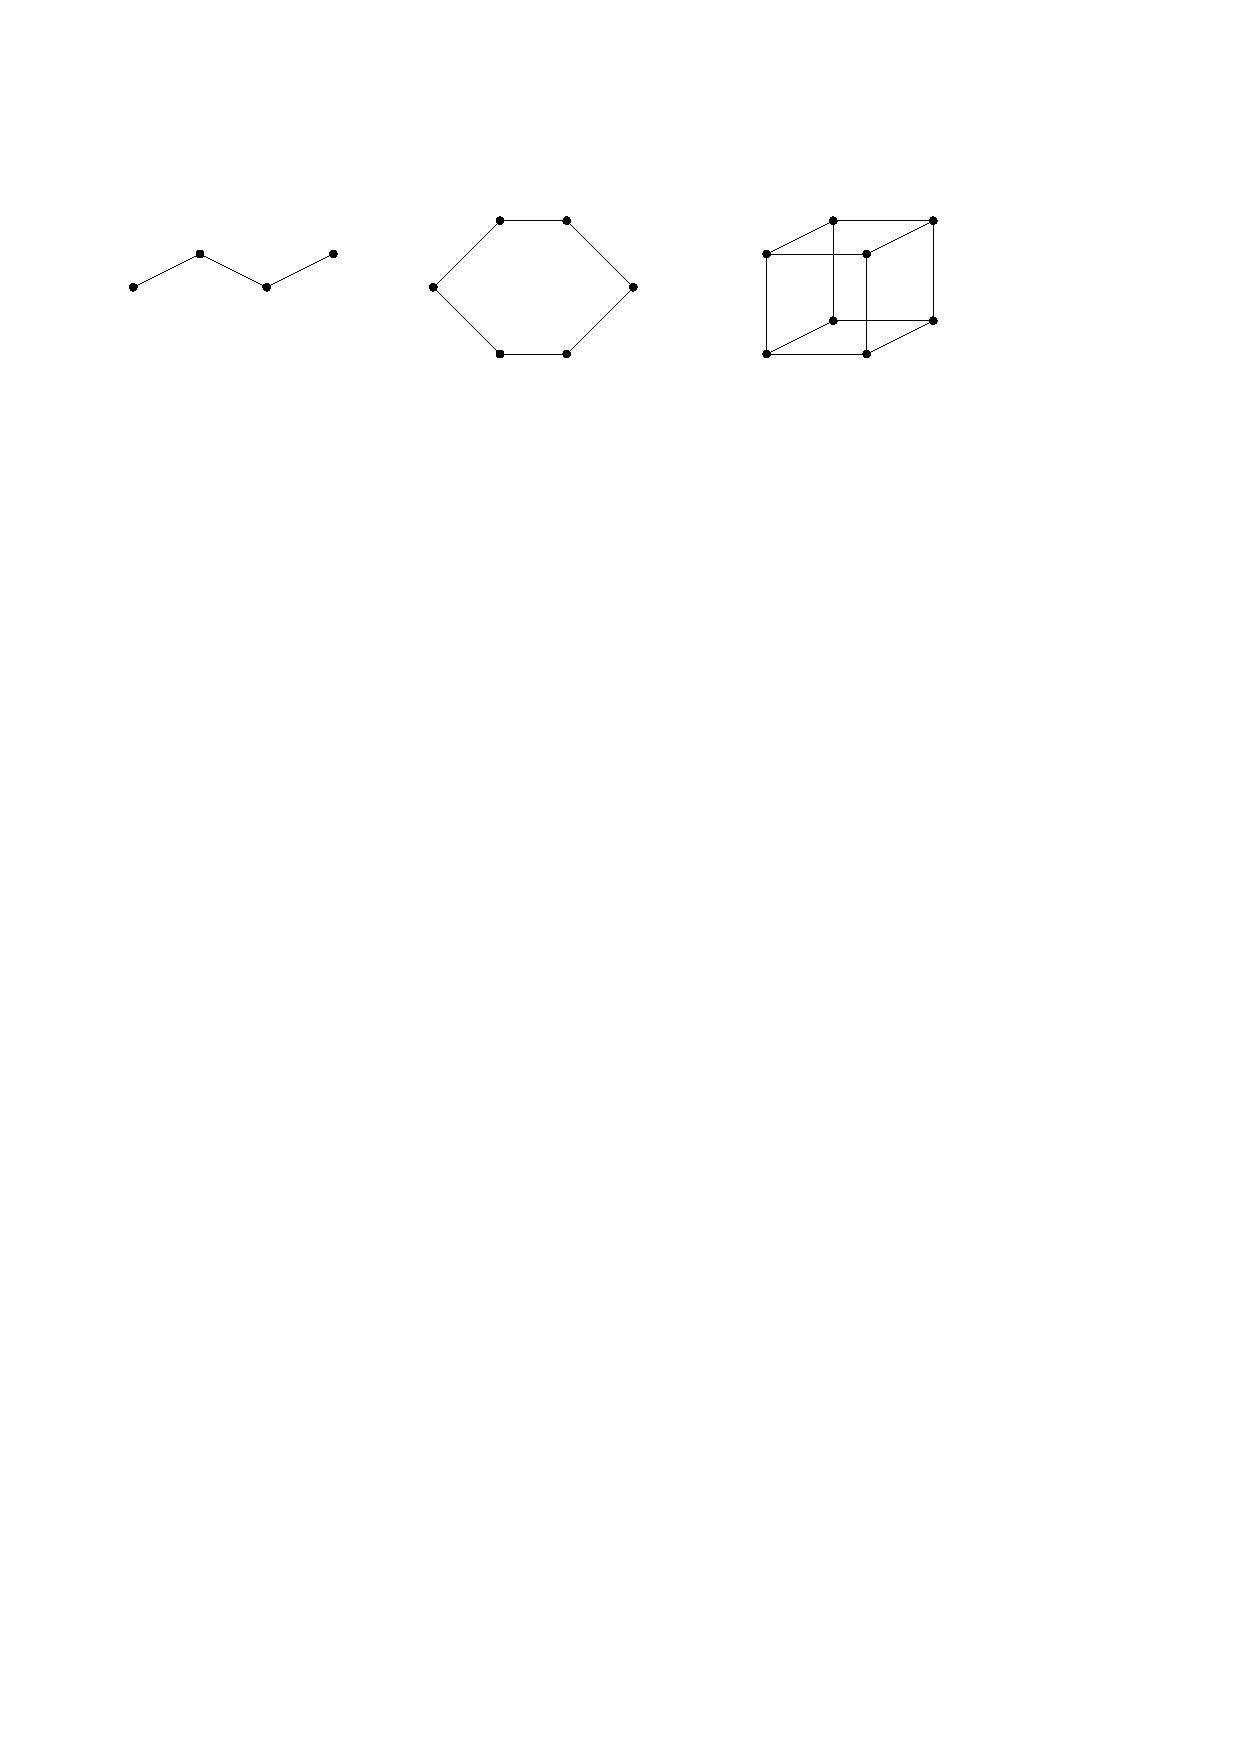
\includegraphics[width=\textwidth]{figures/graphs-number-of-automorphisms.pdf}
\end{center}
Justify your answer!
\end{exercise}
\begin{solution}
	We add numbers as marks to the figure above for convenience of demonstration.
	\begin{enumerate}
		\item For the first graph, this is an easy problem. There are only 4 vertices, among which 1 and 4's degree is one, and 2 and 3's degree is two. If we want to find a function $f: V \rightarrow V$ to satisfy the definition of isomorphism, then the preimage and refletion must have the same degree. Therefore there are \textbf{2 automorphisms}  in this graph, the first one is itself, the second one satisfies the function $f: 1\rightarrow 4, 2\rightarrow3, 3\rightarrow2, 4\rightarrow1$. 
		\item This time every vertex has degree of 2, so the former classfication is no longer userful. But take a close observation of how a graph is completely determined, we can see that once an edge of the hexagon is determined, there is no second choice of how other vertices should be placed. For example, if 1 and 2 are fixed where it is in the figure above, then 6 and 3 must also be at their places in the figure for the limitition of the edges, then the same for 4 and 5. 
		
		Without loss of generosity, let us just consider where to ``place'' vertices 1 and 2, i.e. which vertices to reflect 1 and 2 to. First 1 can be at all six positions, and for each position 1 is at, 2 can either be at the clockwise or anticlockwise adjacent position. And that completes all situations, since there are no other positions 1 can go to and as we have just pointed out that an edge fully determines a graph. Therefore there are $6\times2=$ \textbf{12 automorphisms}  in this graph.
		\item For the last graph it is similar to the second one, but this time we need 2 edges that share one same vertex to fully determine the graph. For example, say 1,2,4 are fixed at positions in the figure above. Each vertex's degree is 3, so the last vertex that is adjacent to 1, 5, must be at its position in the figure. 2 and 4 are both adjcacent to 3, so 3 must be fixed at its place. Now two neighbors of 2 and 4 is determined, so 6 and 8 are also fixed. Only one position is left, that's where 7 should go.
		
		Without loss of generosity, let us just consider where to ``place'' vertices 1, 2 and 4, i.e. which vertices to reflect 1, 2 and 4 to. 1 can be at all eight positions, for each position 2 has 3 according positions, and for each according position of 2, 4 has two positions to choose. Therefore there are $8\times3\times2=$ \textbf{48 automorphisms} in this graph.   
	\end{enumerate}
\end{solution}

For a graph $G = (V,E)$, let $\bar{G} := \left(V, {V \choose 2} \setminus E \right)$ denote
its {\em complement graph}.
\begin{center}
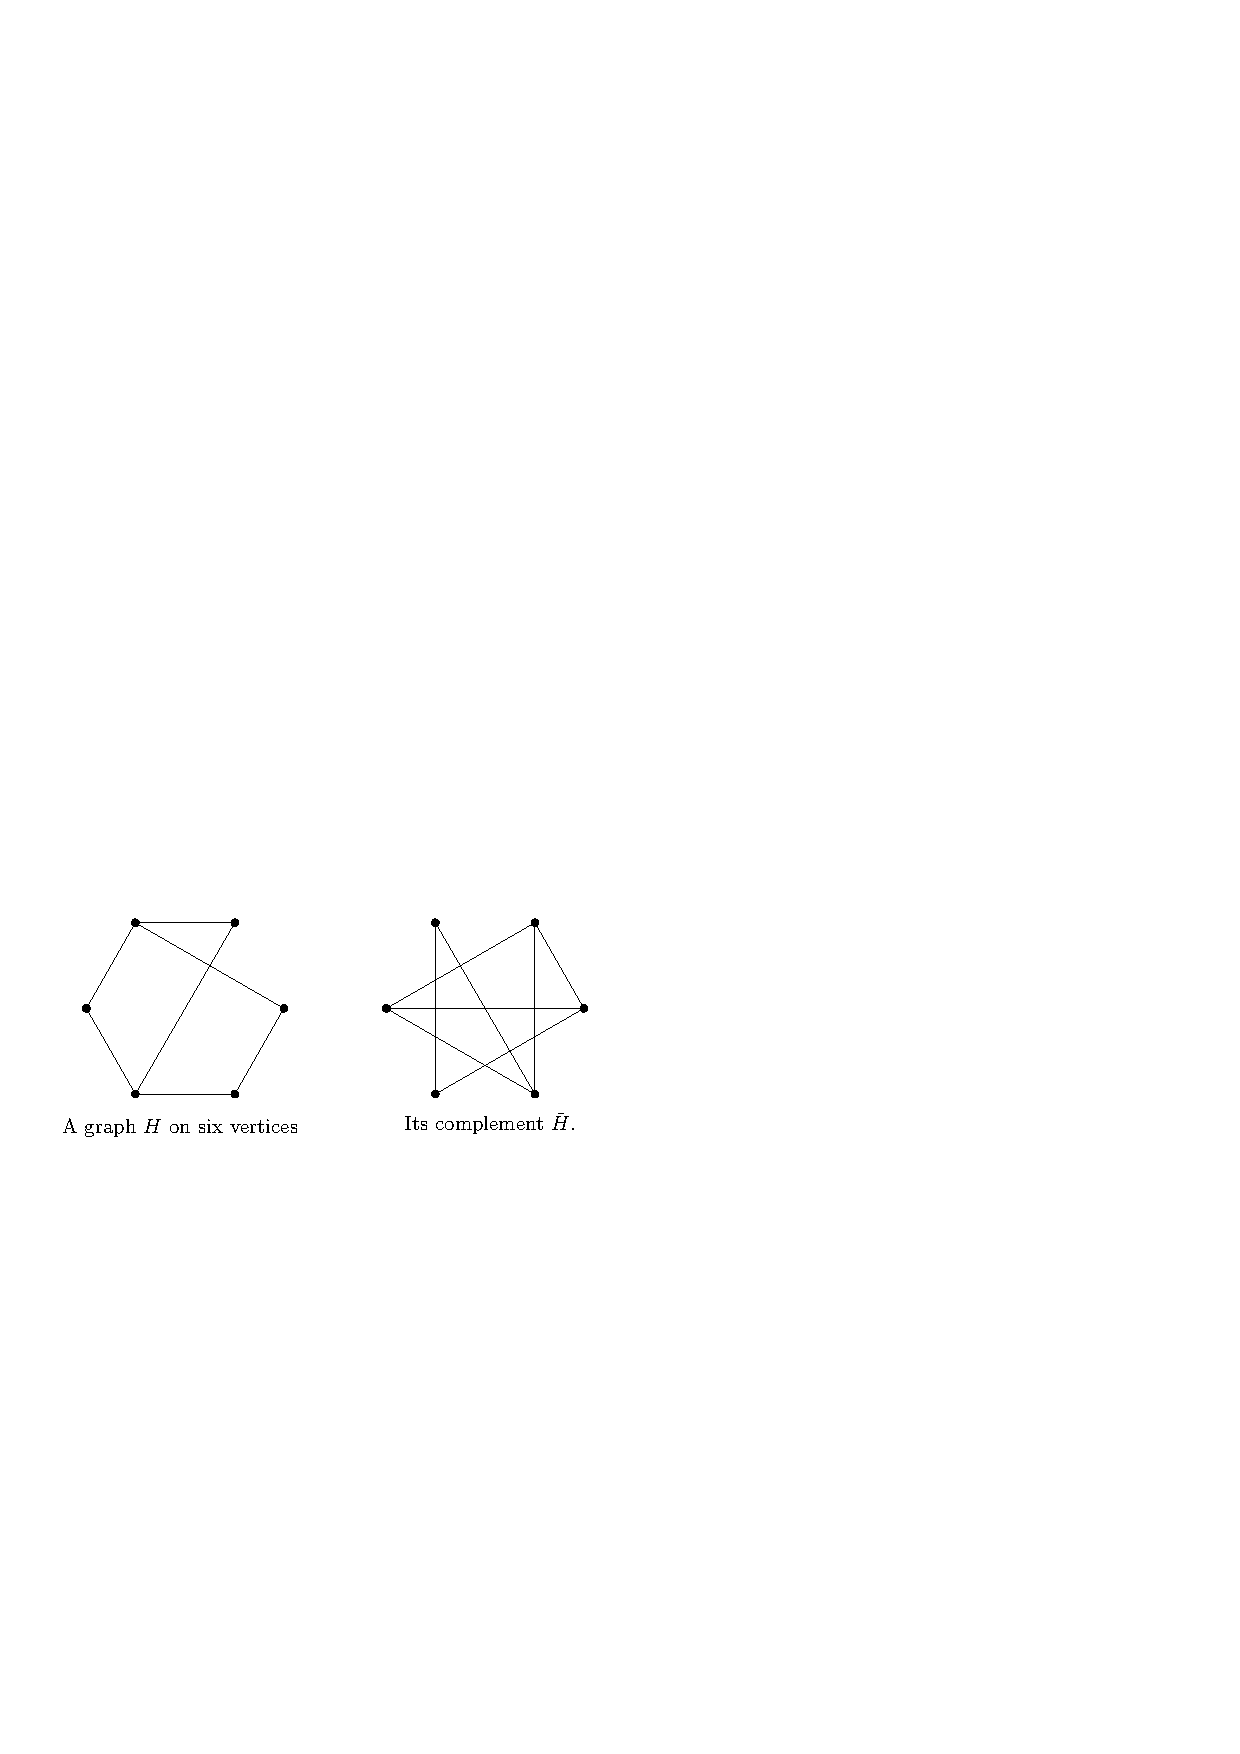
\includegraphics[width=0.5\textwidth]{figures/graph-complement.pdf}
\end{center}
We call a graph {\em self-complementary} if $G \cong \bar{G}$. The above graph
is not self-complementary. Here is an example of a self-complementary graph:
\begin{center}
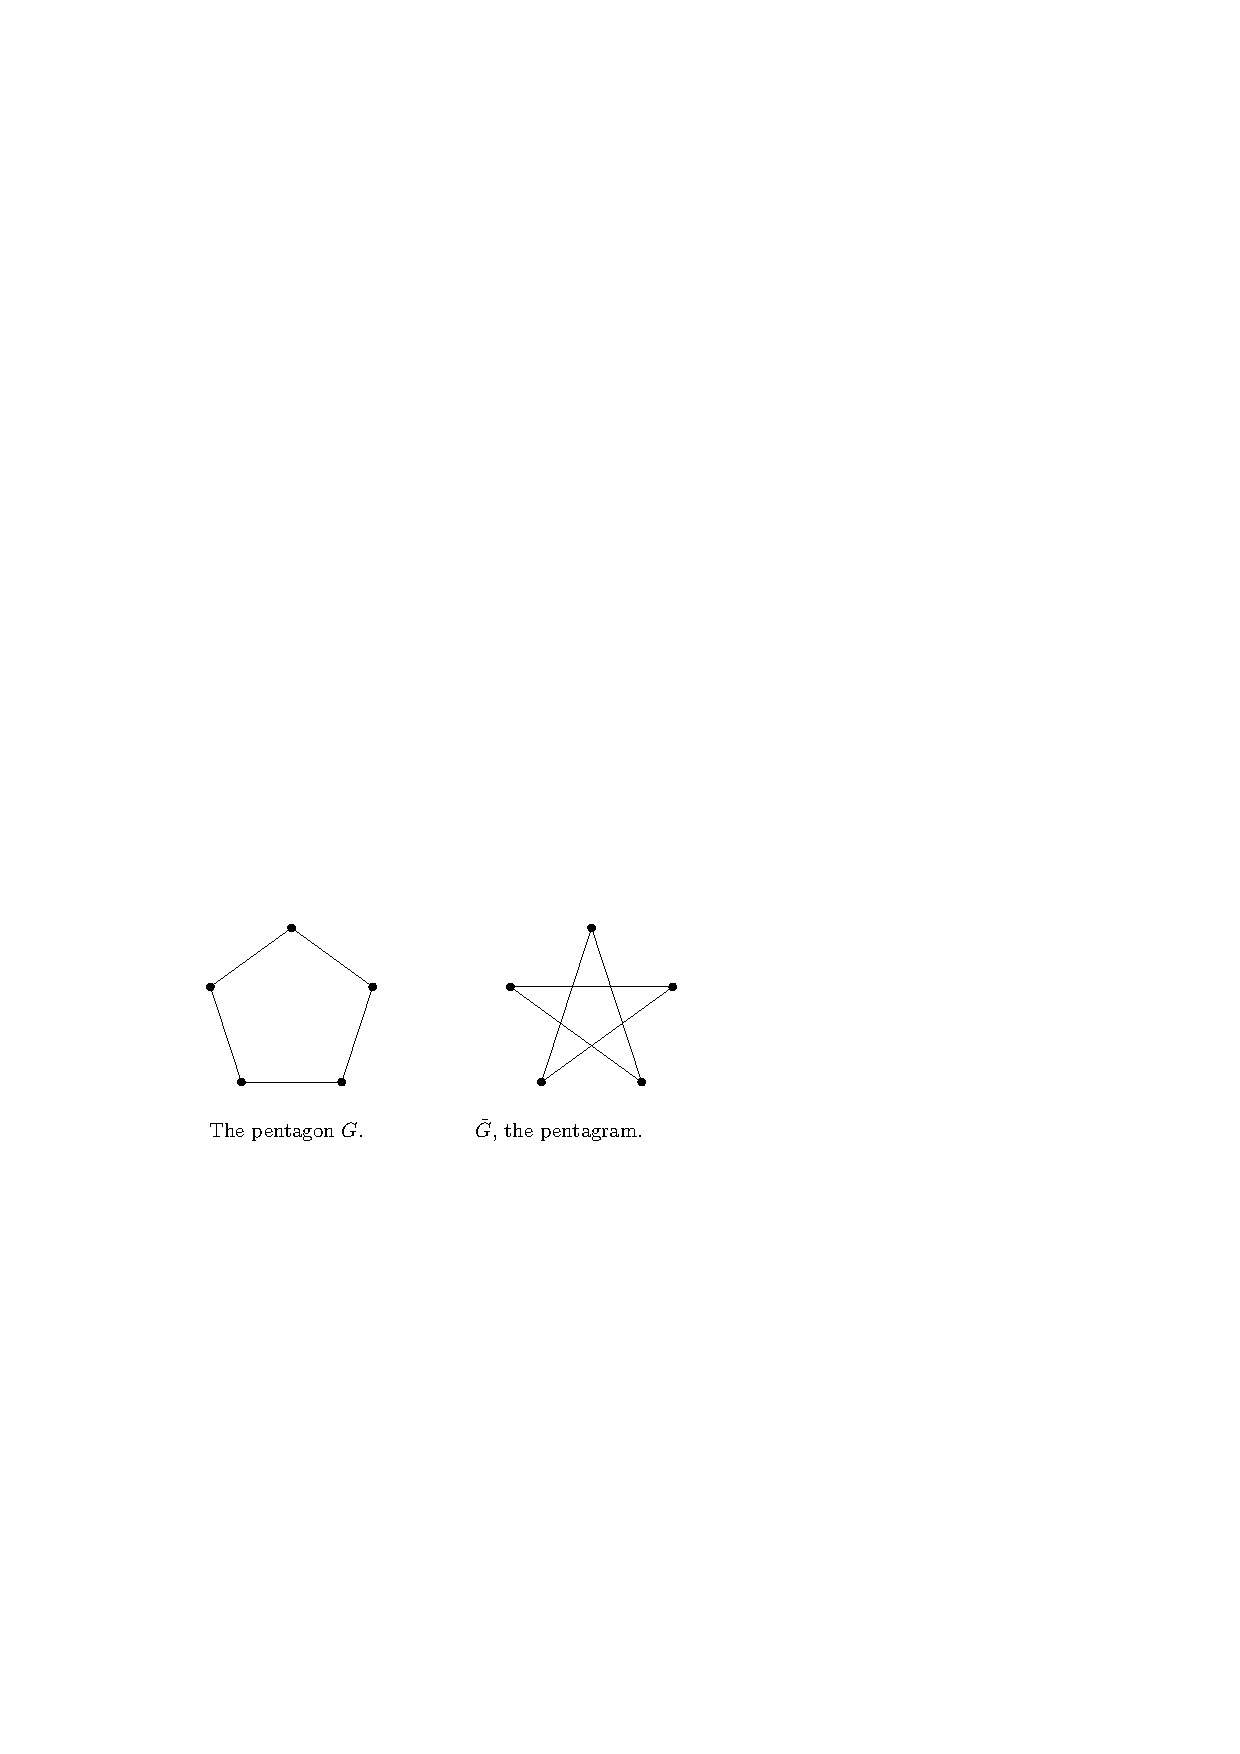
\includegraphics[width=0.5\textwidth]{figures/pentagon-pentagram.pdf}
\end{center}


\begin{exercise}
   Show that there is no self-complementary graph on $999$ vertices.
\end{exercise}

\begin{proof}
	If there is a self-complementary graph on n vertices, $\left|E(K_n)\right|$ must be even. However, for $999$ vertices, we have $\left|E(K_n)\right|$ equal to ${999 \choose 2} = 498501$, which is odd.
\end{proof}

\begin{exercise}
 Characterize the natural numbers $n$ for which there is a self-complementary
 graph $G$ on $n$ vertices. That is, state and prove a theorem of the form
 ``There is a self-complementary graph  on $n$ vertices if and only if 
 $n$ \texttt{ <put some simple criterion here>}.''
\end{exercise}

\begin{solution} \quad
	\item
	\qquad \textbf{theorem.} There is a self-complementary graph on $n$ vertices if and only if $n = 4k \text{ or } 4k + 1$, with $k \in \mathbf{Z^+}$. 

	\begin{proof} \quad
		\item $\rightarrow$: Since $G \cup \bar{G} = K_n$, and $\left|E(K_n)\right| = {n \choose 2}$, we must have $\left|E(G)\right| = \left|E(\bar{G})\right| = \frac{1}{2}{n \choose 2} = \frac{n(n-1)}{4}$. With this integer, we must either have $4 \mid n \text{ or } 4 \mid n - 1$.
		\item $\leftarrow$: We can construct a self-comlementary graph on $4k$ or $4k + 1$ vertices by recurrence. \par
		\begin{enumerate}
			\item Let $Sc$ be any graph which is self-complementary, and let $P_4 = v_1v_2v_3v_4$ be a 4-path, i.e., a path with exactly $4$ vertices. 
			\item Join each of v 2 and v 3 to all vertices of H. We call this operation a 4-path addition.
			\begin{center}
			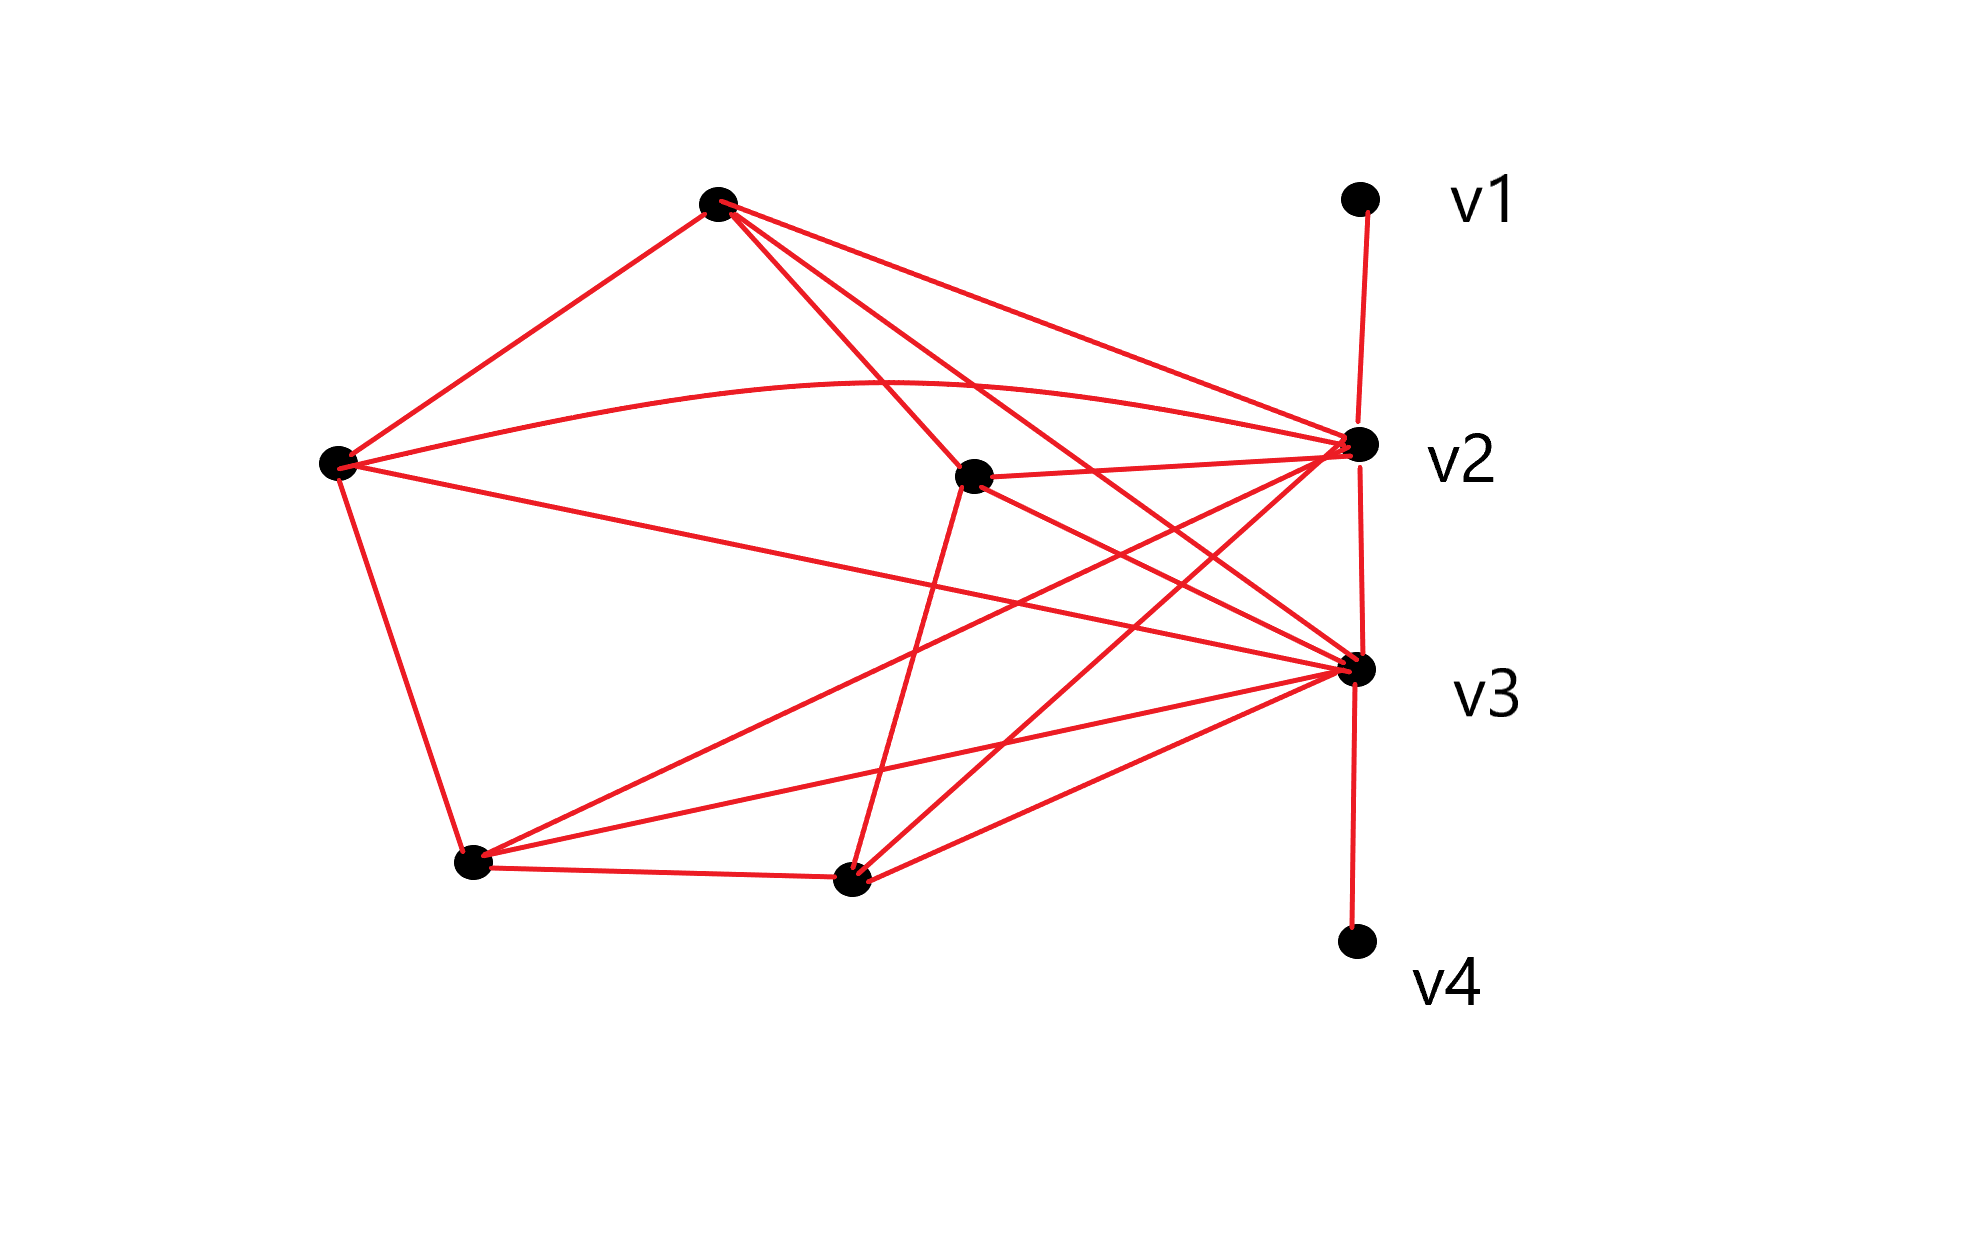
\includegraphics[width=0.5\textwidth]{figures/sc_5.png}
			\end{center}
			 \par
			The resulting graph with $v(H) + 4$ vertices can easily be checked to be self-complementary. Thus, for each $n = 4k$ or $4k + 1$, we can inductively construct self-complementary graph.
			\begin{center}
			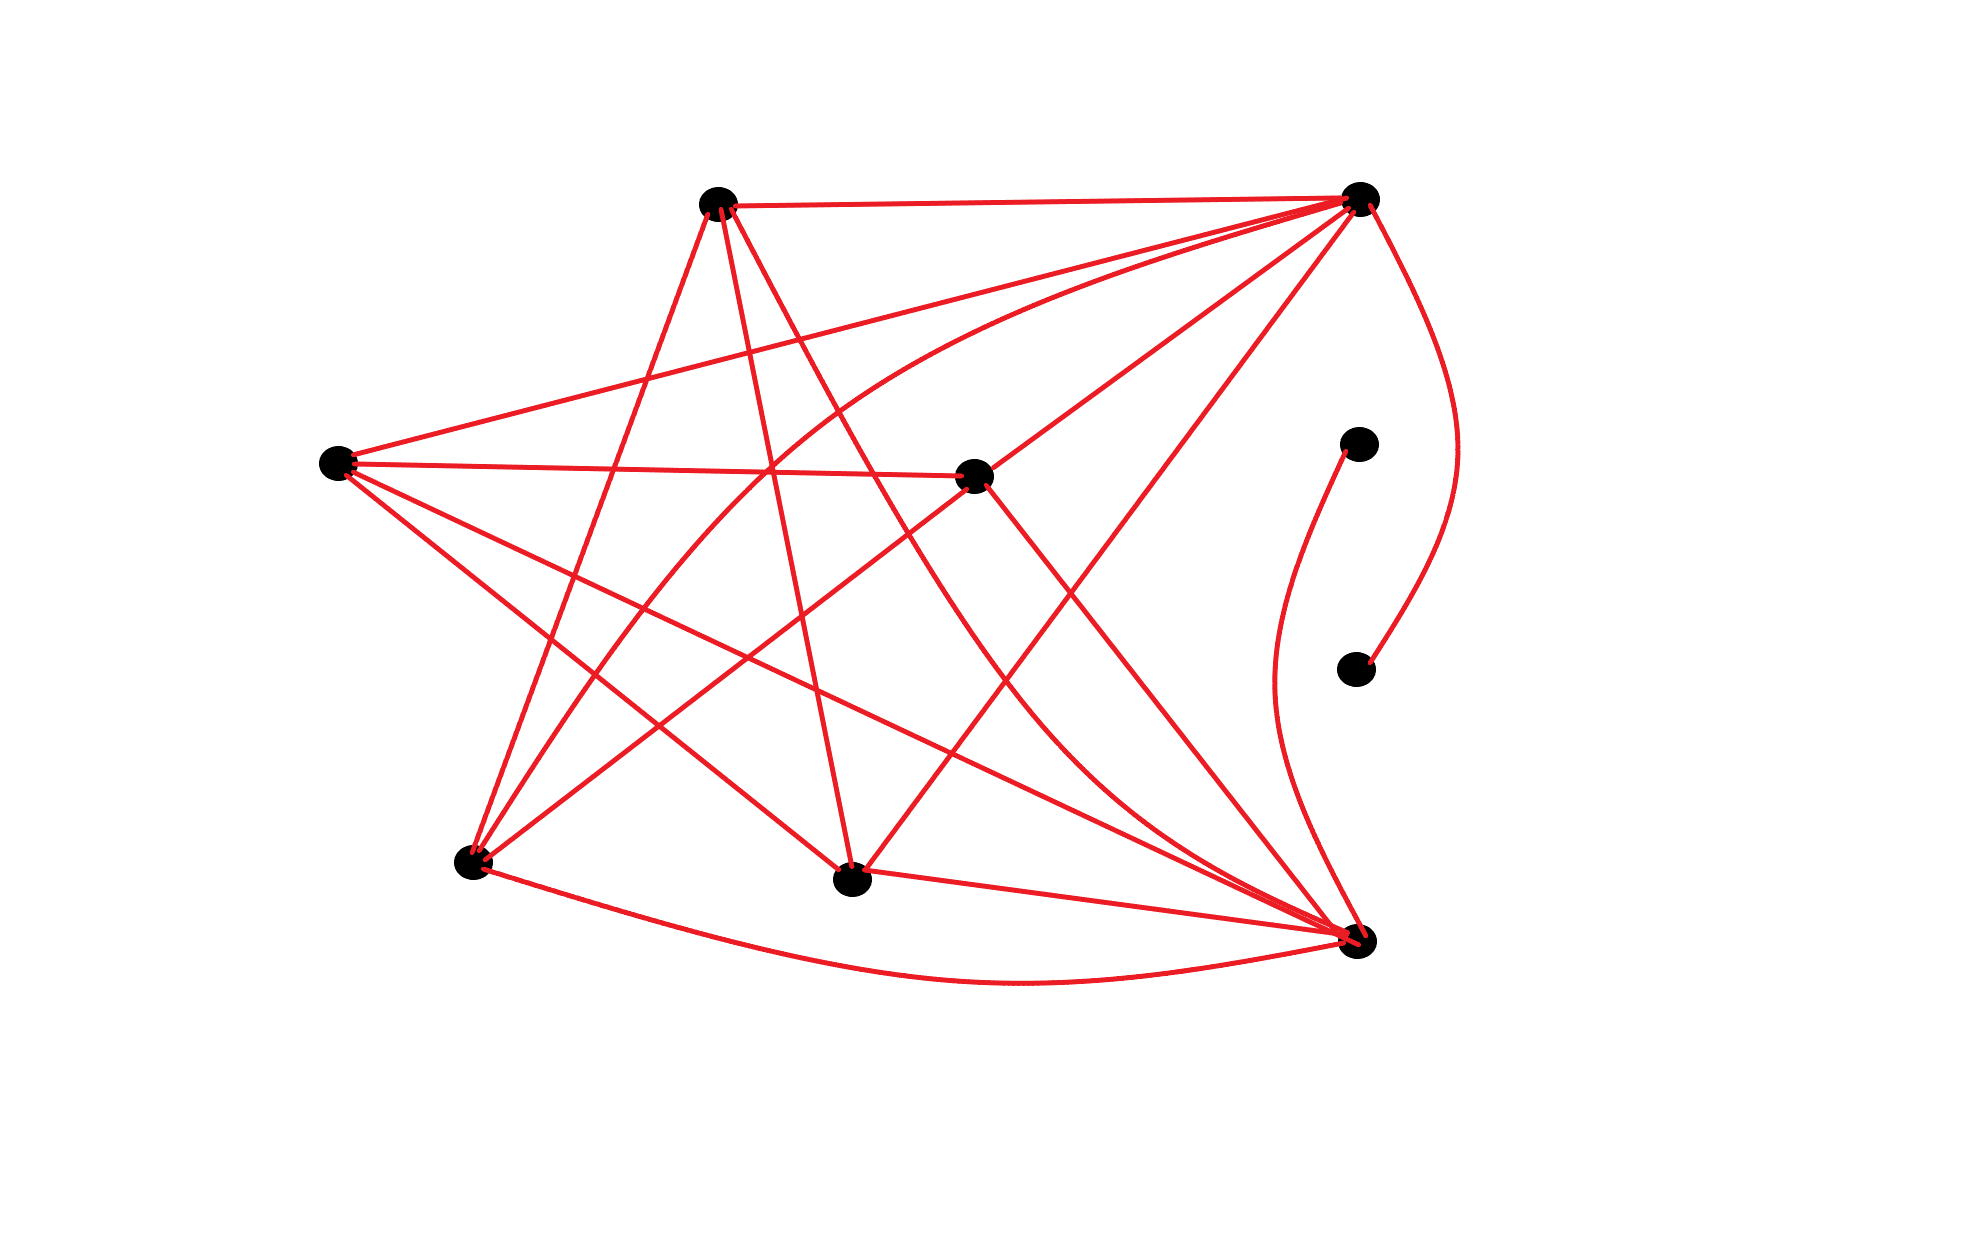
\includegraphics[width=0.5\textwidth]{figures/sc_5_1.png}
			\end{center}
		\end{enumerate}

	\end{proof}

\end{solution}


\begin{exercise}
   Show that for every $k \in \N$, there is some graph $G=(V,E)$ with exactly 
   $k$ automorphisms. \textbf{Hint.} Start with $k=3$. Once you get this, the rest is somewhat easy.
\end{exercise}

\begin{proof}
  \begin{figure}[!htb]
  \centering
  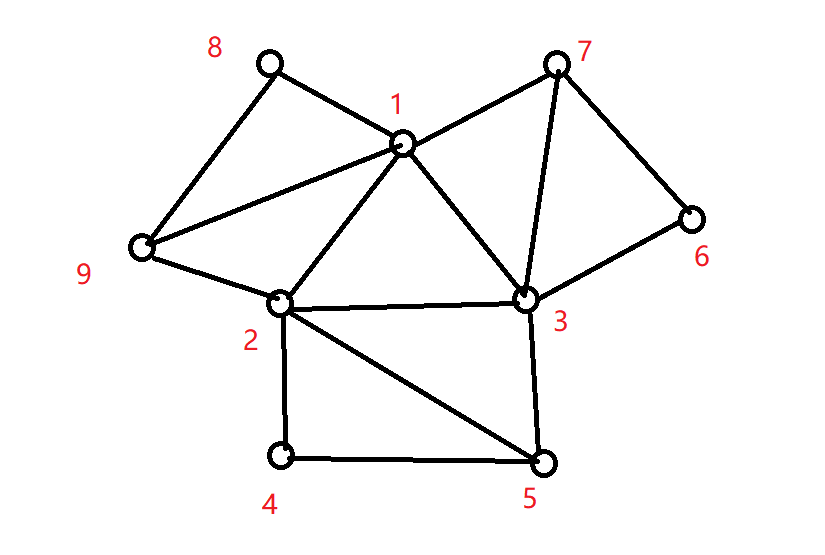
\includegraphics[width=0.5\textwidth]{figures/3.jpg}
  \caption{Graph with 3 automorphisms}\label{3}
\end{figure}
  When $k=3$, the graph is shown as Figure \ref{3}. Rotate it and we can obtain 3 automorphisms.
  When $k=4$, we can the middle triangle into square and get Figure \ref{4}.
  \begin{figure}[htbp]
  \centering
  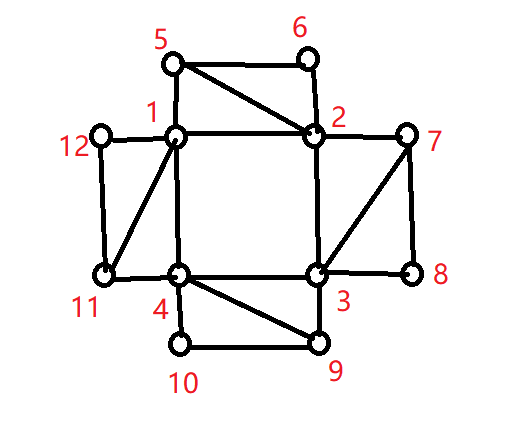
\includegraphics[width=0.5\textwidth]{figures/4.jpg}
  \caption{Graph with 4 automorphisms}\label{4}
\end{figure}
  Similarly, we can get a graph which have exactly $k(k \ge 5)$ automorphisms.
\end{proof}


\begin{exercise}
   Show that for every $n \geq 6$, there is an asymmetric graph on $n$ vertices.
      \label{exercise-aut-every-n}
\end{exercise}
%---------------------------BEGIN---------------------------
\textbf{Solution.} If $n=6$, we can easily find asymmetric graphs on $n$ vertices. An example is shown in figure \ref{ex651}. \\
	\begin{figure}[htbp]
	    \centering
        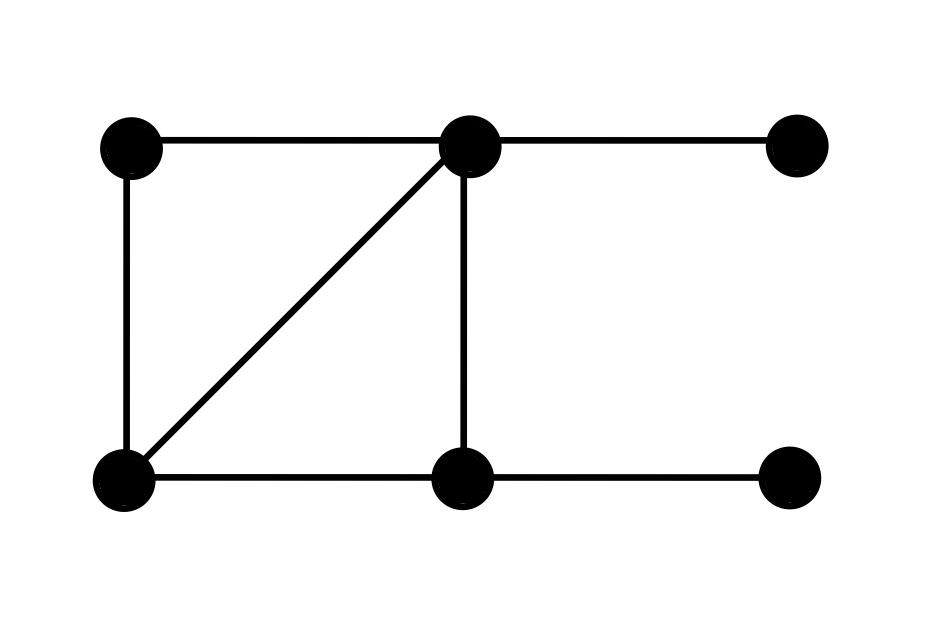
\includegraphics[width=0.4\textwidth]{figures/651.jpeg}
        \caption{An example of asymmetric graph on 6 vertices}
        \label{ex651}
	\end{figure}\\
	Based on $6$ vertices, we can add more vertices on figure \ref{ex651} and get an asymmetric graph on arbitrary number of vertices. The asymmetric graph with $n$ vertices is shown in figure \ref{ex652}.
	\begin{figure}[htbp]
	    \centering
        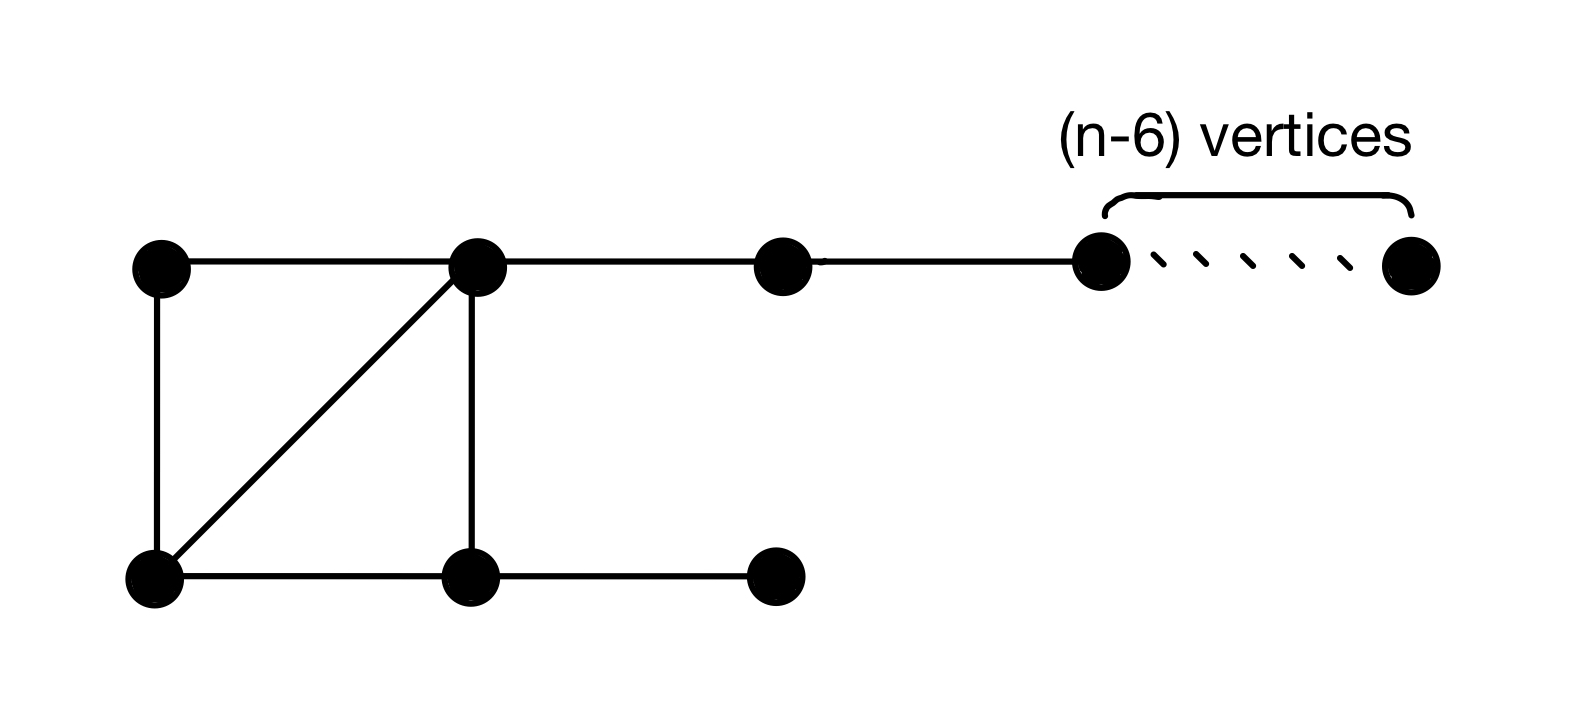
\includegraphics[width=0.7\textwidth]{figures/652.jpg}
        \caption{An example of asymmetric graph on n vertices}
        \label{ex652}
	\end{figure}\\
	Therefore, there is at least one asymmetric graph on $n$ vertices when $n \geq 6$.
%----------------------------END----------------------------

\begin{exercise}
  Show that for every ``sufficiently large $n$'' (I guess $n \geq 6$ works), there is a graph on
  $3n$ vertices with {\em exactly} $2^n$ automorphisms.
\end{exercise}

%---------------------------BEGIN---------------------------
\textbf{Solution.} From Exercise 6.5, we know if $n \geq 6$, then there is at least one asymmetric graph on $n$ vertices. For an asymmetric graph on $n$ vertices shown in \ref{ex652}, we add two leaf vertices on each vertex of this graph, which is shown in figure \ref{ex66}.\\
	\begin{figure}[htbp]
	    \centering
        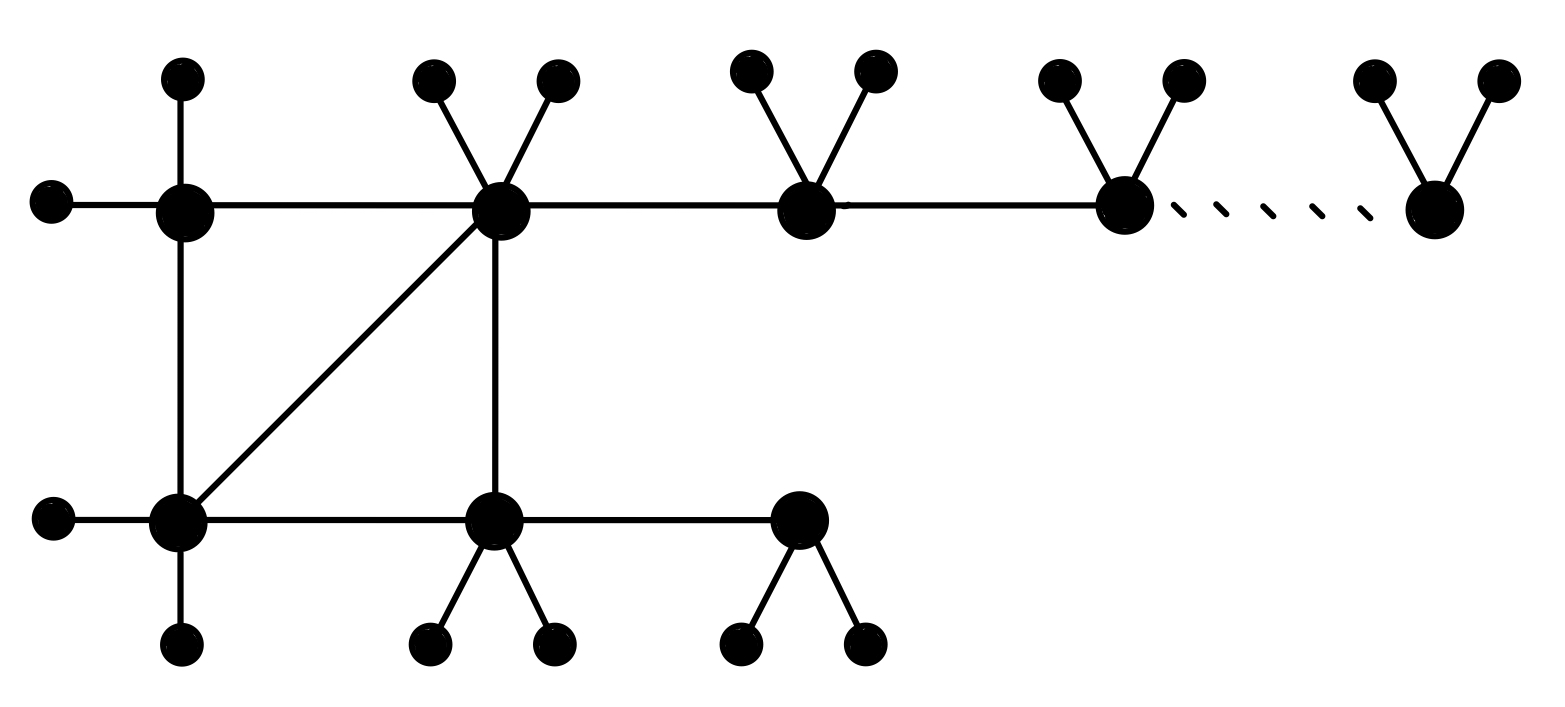
\includegraphics[width=0.73\textwidth]{figures/66.jpeg}
        \caption{An example of asymmetric graph on 6 vertices}
        \label{ex66}
	\end{figure}\\
	The total number of vertices of this graph is $3n$. Also, because each pair of two leaf vertices doubles the number of automorphisms of this graph, the total number of automorphisms of this graph is exactly $2^n$.
%----------------------------END----------------------------

\begin{exercise}
 Let $p \geq 7$ be a prime. From Exercise~\ref{exercise-aut-every-n}, we know that there 
 is a graph with exactly $p$ automorphisms. However, this graph (at least in my construction)
 has roughly $6p$ vertices. Can you do better? Can you find such a graph on $O(\sqrt{p})$ vertices?
 Or even $O(\log(p))$ vertices? \textbf{Warning:} I don't know the answer; this might be very hard.
 \end{exercise}





\end{document}